\chapter{Stand der Wissenschaft und Technik}
\label{chap:stand}
% Inhalt (Gliederung Kapitel 2, etwa 16 S., aus BA-0486 Kapitel 2 neu geordnet): Bilder nur aus
% Quellen "nach [..]", aus CADMOULD oder dem FVA-Bericht; eigene Bilder nur die
% Stommel-Methodenbilder für PA46-GF30 "in Anlehnung an [Sto18]".

\section{Thermoplaste als Zahnradwerkstoff}
\label{sec:thermoplaste}
% Inhalt: Einordnung, Temperatur, Feuchte, Dehnrate, Kurzglasfasern, Stanyl TW200F6,
% Vergleichswerkstoffe POM und PEEK. Quellen VDI 2736 Blatt 1, Ehrenstein, Erhard,
% Erhard/Strickle, Stommel Kap. 2, CAMPUS-Datenblatt, Illenberger, MA-0296 4.2.1. BA 2.1, 2.2.1.
% Tabelle Kennwerte aus Datenblatt und Matscape-Karten.

\section{Spritzgießen und Faserorientierung}
\label{sec:spritzgiessen}
% Inhalt: Spritzgießen von Zahnrädern, Orientierungstensor, Anisotropie-Index, Zonenmodell und
% CT-Befund FVA 856 I, Prozess-Struktur-Kopplung als Prinzip. Quellen FVA 856 I Kap. 6, VDI 2736
% Blatt 1, Kassem 2022/2023. Bilder: CADMOULD Füllung und Orientierung, FVA 856 I Bild 16/17/18.
\Note{PH: CADMOULD-Bilder der Füllung und Orientierung (Nutzer legt ab).}

\section{Werkstoffverhalten und Materialmodelle}
\label{sec:materialmodelle}
% Inhalt: Zugversuch nach Richtung, Rate und Temperatur; isotrop linear, elastisch-plastisch,
% orthotrop, Hill; Herleitung der Werkstoffstufen W1 bis W4. Quellen Stommel Kap. 2, Abaqus-Doku,
% FVA 856 I Tab. 4, METG-Kurven. BA 2.2.2. Bilder stommel_methode_V2/spannung_dehnung_*,
% orientierungszustaende_*; Tabelle Tab. 4.

\section{Zahnradschäden und Zahnfußtragfähigkeit}
\label{sec:schaeden}
% Inhalt: Schadensarten, 30°-Tangente, Versagensdefinitionen, Einflüsse. Quellen VDI 2736 Blatt 2,
% Hasl, Illenberger, MA-0296, Klocke/Brecher, Linke. BA 2.2.3. Quellbilder mit Verweis.

\section{Berechnung der Zahnfußbeanspruchung}
\label{sec:berechnung_stand}
% Inhalt: 5 S., BA 2.3.1 bis 2.3.3 (Formeln am gerenderten Buch prüfen, K_M nach Gl. 6.21,
% Druckfaktor, Tab. 2.5).

\subsection{Berechnung nach VDI 2736}
\label{sec:vdi2736}
% Inhalt: VDI 2736 Blatt 2 mit Y-Faktoren nach ISO 6336-3 Methode B. Quellen VDI 2736 Blatt 2,
% ISO 6336-1/-3, Niemann/Winter, Linke.

\subsection{Numerische Verfahren und Zahnfußgeometrien}
\label{sec:numerik_fussgeometrien}
% Inhalt: RIKOR, FVA-Workbench, FEM; Fußrundungsvarianten elliptisch (Frühe, Kassem, Landi),
% Bézier (Roth/Opferkuch, Dong), bionisch (Patente), Kassem 2023. Quellen FVA 30 XI/XII, FVA 892 I,
% FVA 484 V, Frühe, Hasl, Kassem, Landi, Dong, Roth/Opferkuch, Sanders, Patente, FVA 241 XII.
% Quellbilder der Fußgeometrien "nach [..]".

\subsection{Bemessung nach Stommel et al.}
\label{sec:stommel_stand}
% Inhalt: statisch, zyklisch, Überlastfälle, Isotropie-Vorschrift, Erweiterungsbasis. Quelle
% Stommel Kap. 6. Eigene Methodenbilder nomogramm_qs, haigh_qs_80C, woehler_synthetisch_qs
% "in Anlehnung an [Sto18]".
\Note{PH: Text zu 2.5.3 folgt (aus BA-0486 2.3.3, am Buch geprüft); die beiden Methodenbilder stehen schon hier, weil 3.7 auf sie verweist.}

\begin{figure}[htbp]
    \centering
    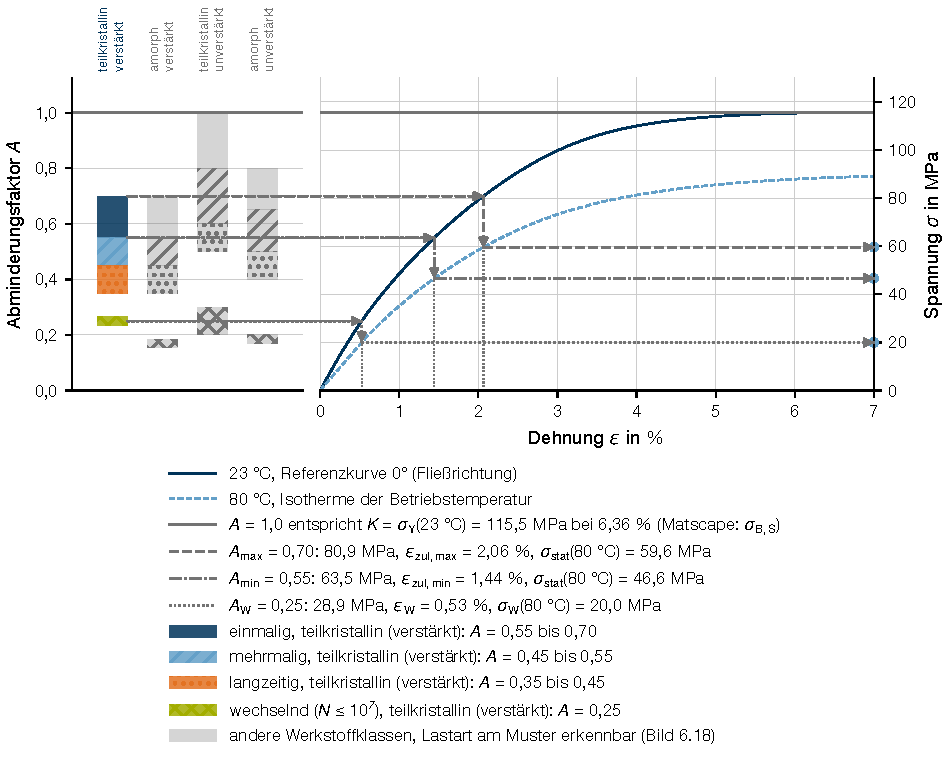
\includegraphics[width=0.85\textwidth]{kap2/nomogramm_qs}
    \caption{Nomogramm der statischen Bemessung nach Stommel et al. für PA46-GF30 mit der quasistatischen Werkstoffkarte, in Anlehnung an \cite{Sto18}.}
    \label{fig:nomogramm_qs}
\end{figure}

\begin{figure}[htbp]
    \centering
    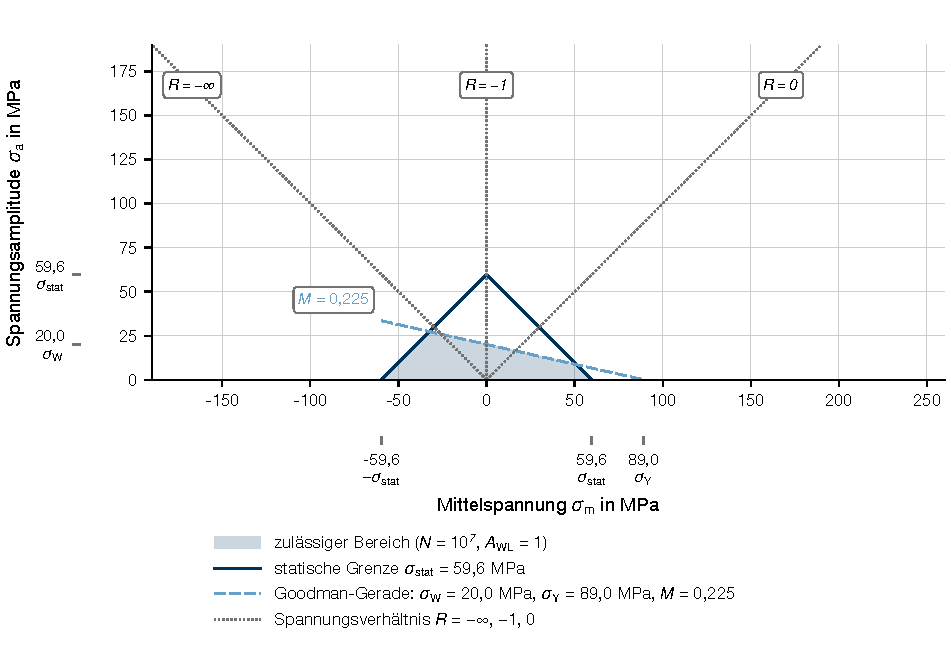
\includegraphics[width=0.85\textwidth]{kap2/haigh_qs_80C}
    \caption{Haigh-Diagramm der zyklischen Bemessung für PA46-GF30 bei $80$\,\textdegree C mit der quasistatischen Werkstoffkarte, in Anlehnung an \cite{Sto18}.}
    \label{fig:haigh_qs_80C}
\end{figure}

\section{Experimentelle Tragfähigkeitsermittlung und Statistik}
\label{sec:experiment_stand}
% Inhalt: Laufversuch, Wöhlerlinie ohne Dauerfestigkeit, Belegung, log-Normalverteilung,
% Perlschnur DIN 50100, Weibull, Durchläufer. Quellen DIN 50100, VDI 2736 Blatt 4, Hasl,
% Illenberger, MA-0296 2.2/2.4/2.5. Prinzipbild aus VDI 2736 Blatt 4 oder MA-0296 "nach [..]".

\section{Problemstellung und Zielsetzung}
\label{sec:problemstellung}
% Inhalt: Lücken und Ziele aus 2.1 bis 2.6. BA 2.4. Keine Bilder.
